\chapter{Chapitre \ref{sec:cine1} exercices}
\label{sec:exer_kinematic}

%\subsection{Système de coordonnées}
%
%\subsubsection{Détermination de systèmes de coordonnées pour des systèmes robotiques}
%
%Pour les systèmes robotiques suivants, a) déterminez les coordonnées qui représentes l'espace des joints et ensuite b) déterminez un système de coordonnées qui serait adapté pour décrire la tâche.
%
%\paragraph{A)} 
%
%TODO
%
%
%\paragraph{B)} 
%
%TODO
%
%
%\paragraph{C)} 
%
%TODO


%\subsection{Vecteurs positions}

\section{Traduire des énoncés en équations vectorielles}
\label{sec:exerposmaison}

Convertissez les énoncés suivant en équations vectorielles avec des scalaires qui représentent des distances et des vecteur unitaires qui représentent des directions. 

\paragraph{A)} 

À partir d'un point A, on avance de 100m vers le nord, 15m vers l'ouest et 50m vers le sud-est, pour arriver sur le point B.

\paragraph{B)} 

À partir d'un point A, on avance de 50m vers le sud, dévie de 30 degrés vers la gauche (bâbord) et avance de 100m, pour arriver sur le point B. 


\paragraph{C)} 

À partir d'un point A, on avance de 200m vers le l'est, dévie de 60 degrés vers la droite (tribord) et avance de 50 m. Ensuite, on s'oriente à l'opposé de la direction du point A et on double la distance par rapport au point A pour arriver sur le point B.
 

\section{Substitution de vecteurs unitaires}

Convertissez les équations vectorielles obtenues à l’exercice \ref{sec:exerposmaison} pour seulement contenir les deux vecteurs unitaires suivants:
%%%%%%%%%%%%%%%%%%%%%%%%%%%%%%%%%%%
\begin{align}
\hat{n} : Nord \quad\quad   \hat{o} : Ouest
\end{align} 
%%%%%%%%%%%%%%%%%%%%%%%%%%%%%%%%%%%


%\subsection{Bases vectorielles}

\section{Obtenir les composantes avec un produit scalaire}

Le vecteur $\vec{v}$ est définie dans une base vectorielle orthogonale $a$:
%%%%%%%%%%%%%%%%%%%%%%%%%%%%%%%%%%%
\begin{align}
\vec{v} = v_1 \hat{a}_1 + v_2 \hat{a}_2 + v_3 \hat{a}_3
\end{align} 
%%%%%%%%%%%%%%%%%%%%%%%%%%%%%%%%%%%
démontrez que 
%%%%%%%%%%%%%%%%%%%%%%%%%%%%%%%%%%%
\begin{align}
v_1 = \vec{v} \bullet \hat{a}_1 \\
v_2 = \vec{v} \bullet \hat{a}_2 \\
v_3 = \vec{v} \bullet \hat{a}_3 
\end{align} 
%%%%%%%%%%%%%%%%%%%%%%%%%%%%%%%%%%%
en se basant sur les définitions.


%\subsection{Matrices de rotation}

\section{Matrice de rotation calculée avec toutes les définitions}

Effectuer le calcul de la matrice $R_3$ discutée à la section \ref{sec:rot3}:

\paragraph{A)} À partir de la définition basée sur les produit scalaires:
%%%%%%%%%%%%%%%%%%%%%%%%%%%%%%%%%%%
\begin{align}
R_b^a &= 
\left[ \begin{array}{c c c} 
\hat{a}_1 \bullet \hat{b}_1  &  \hat{a}_1 \bullet \hat{b}_2  &  \hat{a}_1 \bullet \hat{b}_3 \\
\hat{a}_2 \bullet \hat{b}_1  &  \hat{a}_2 \bullet \hat{b}_2  &  \hat{a}_2 \bullet \hat{b}_3 \\
\hat{a}_3 \bullet \hat{b}_1  &  \hat{a}_3 \bullet \hat{b}_2  &  \hat{a}_3 \bullet \hat{b}_3 
\end{array} \right] 
\end{align} 
%%%%%%%%%%%%%%%%%%%%%%%%%%%%%%%%%%%
\paragraph{B)} À partir de la définition basée sur l'angle entre les vecteurs unitaires:
%%%%%%%%%%%%%%%%%%%%%%%%%%%%%%%%%%%
\begin{align}
R_b^a &= 
\left[ \begin{array}{c c c} 
\cos \angle (\hat{a}_1 , \hat{b}_1)  &  \cos \angle (\hat{a}_1 , \hat{b}_2)  &  \cos \angle (\hat{a}_1 , \hat{b}_3) \\
\cos \angle (\hat{a}_2 , \hat{b}_1)  &  \cos \angle (\hat{a}_2 , \hat{b}_2)  &  \cos \angle (\hat{a}_2 , \hat{b}_3) \\
\cos \angle (\hat{a}_3 , \hat{b}_1)  &  \cos \angle (\hat{a}_3 , \hat{b}_2)  &  \cos \angle (\hat{a}_3 , \hat{b}_3) 
\end{array} \right] 
\end{align} 
%%%%%%%%%%%%%%%%%%%%%%%%%%%%%%%%%%%
\paragraph{C)} À partir de la définition basée sur les composants des vecteurs unitaires $\hat{b}_i$ dans la base $a$:
%%%%%%%%%%%%%%%%%%%%%%%%%%%%%%%%%%%
\begin{align}
R_b^a &= 
\left[ \begin{array}{c c c} 
\col{b}_1^a &  \col{b}_2^a & \col{b}_3^a
\end{array} \right] 
\end{align} 
%%%%%%%%%%%%%%%%%%%%%%%%%%%%%%%%%%%
\paragraph{D)} À partir de la définition basée sur les composants des vecteurs unitaires $\hat{a}_i$ dans la base $b$:
%%%%%%%%%%%%%%%%%%%%%%%%%%%%%%%%%%%
\begin{align}
R_b^a &= 
\left[ \begin{array}{c} 
(\col{a}_1^b)^T \\
(\col{a}_2^b)^T \\
(\col{a}_3^b)^T
\end{array} \right] 
\end{align} 
%%%%%%%%%%%%%%%%%%%%%%%%%%%%%%%%%%%
\paragraph{E)} À partir de la définition basée sur les angles de Euler:
%%%%%%%%%%%%%%%%%%%%%%%%%%%%%%%%%%%
\begin{align}
R_b^a &= 
\left[ \begin{array}{c c c}
	 + c\phi \, c\psi - s\phi\,c\theta\,c\psi  & - c\phi \, s\psi - s\phi \, c\theta c\psi  & + s\phi \, s\theta  \\
	 + s\phi \, c\psi + c\phi\,c\theta\,c\psi  & - s\phi \, s\psi + c\phi \, c\theta c\psi  & - c\phi \, s\theta  \\
	 + s\theta \, s\psi                        & + s\theta \, c\psi                          & + c\theta 
\end{array}  \right]
\end{align} 
%%%%%%%%%%%%%%%%%%%%%%%%%%%%%%%%%%%



\section{Axe de rotation à partir d'une matrice de rotation}

La figure \ref{fig:exer_mat_axe_1} illustre deux base vectorielle avec une orientation relative décrite par la matrice ${}^aR^b$. 
%%%%%%%%%%%%%%%%%%%%%
\begin{figure}[H]
	\centering
		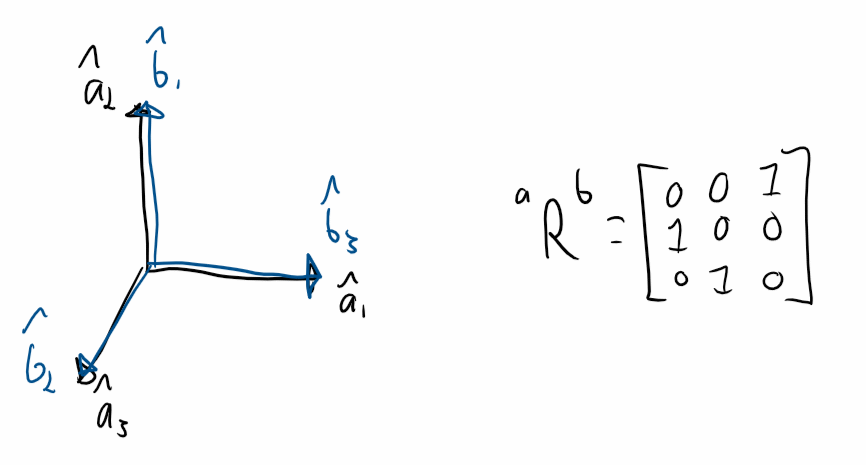
\includegraphics[width=0.40\textwidth]{exer_mat_axe_1.png}
	\caption{Calcul d'un axe de rotation à partir d'une matrice}
	\label{fig:exer_mat_axe_1}
\end{figure}
%%%%%%%%%%%%%%%%%%%%%%

\paragraph{A)} Vérifiez que la matrice de rotation illustrée ci-dessus a une valeur propre réel $\lambda=1$.
\paragraph{B)} Calculez le vecteur propre associé.
\paragraph{C)} Vérifiez graphiquement que le vecteur propre calculé correspond à l’axe de rotation.


%%%%%%%%%%%%%%%%%%%%%%%%%%%%%%%%%%%%%%%%%%%%%%%%%%%%%%%
\section{Fonction pour un changement de repère}

Un avion détecte un ovni et sa position dans son repère $\{ V_o, \hat{v}_1, \hat{v}_2, \hat{v}_2\}$, il doit transmettre les coordonnées de cet ovni par rapport au repère $\{ B_o, \hat{b}_1, \hat{b}_2, \hat{b}_2\}$ de la base, voir figure \ref{fig:exrep}. Écrivez une fonction, dans votre langage de programmation préféré, pour effectuer le calcul:
%%%%%%%%%%%%%%%%%%%%%%%%%%%%%%%%%%%
\begin{align}
\col{r}^b_{Ovni/B_o} = f\left( \col{r}^v_{Ovni/V_o}, \theta, h, d\right)
\end{align} 
%%%%%%%%%%%%%%%%%%%%%%%%%%%%%%%%%%%
%%%%%%%%%%%%%%%%%%%%%
\begin{figure}[H]
	\centering
		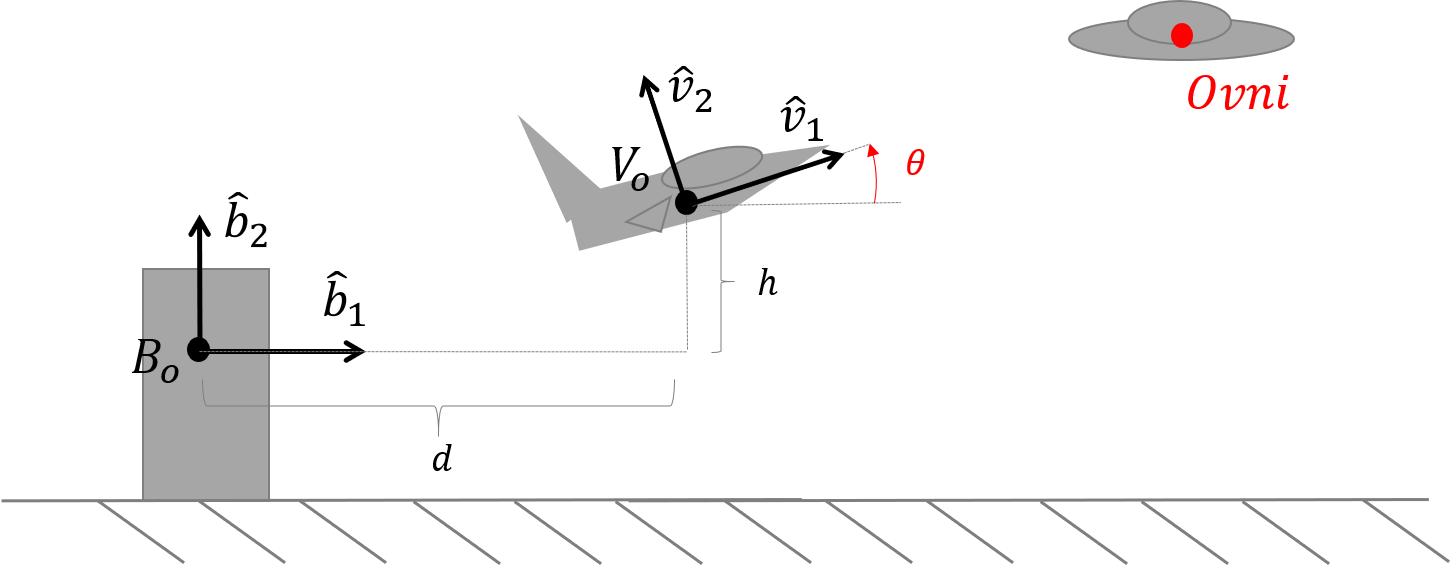
\includegraphics[width=0.70\textwidth]{exrep.png}
	\caption{Calcul d'un changement de repère}
	\label{fig:exrep}
\end{figure}
%%%%%%%%%%%%%%%%%%%%%%


%%%%%%%%%%%%%%%%%%%%%%%%%%%%%%%%%%%%%%%%%%%%%%%%%%%%%%%
\section{Calcul de la cinématique d'un robot à deux joints}

La figure \ref{fig:exrobot2} illustre un robot planaire à deux joints. 
%%%%%%%%%%%%%%%%%%%%%
\begin{figure}[H]
	\centering
		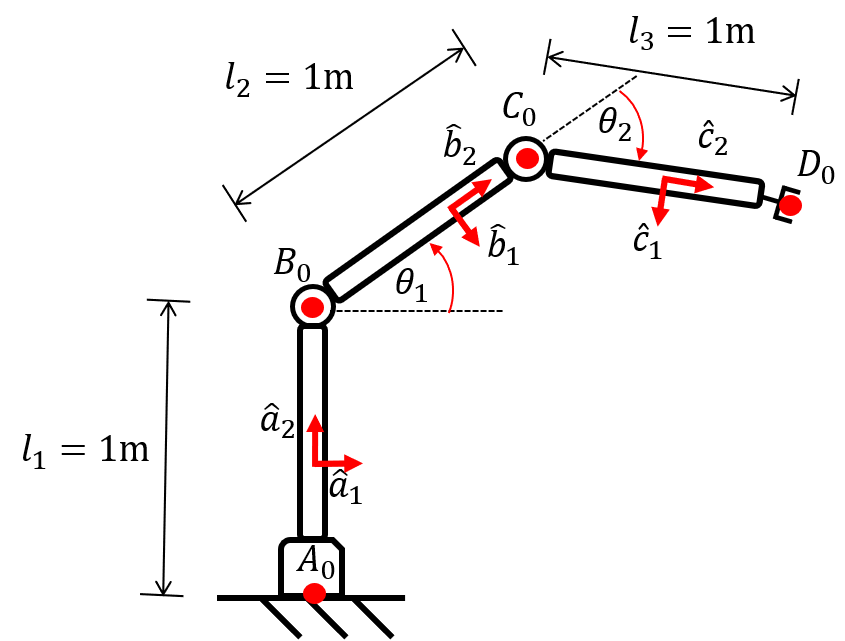
\includegraphics[width=0.50\textwidth]{exrobot2.png}
	\caption{Calcul de la cinématique d'un robot à deux joints}
	\label{fig:exrobot2}
\end{figure}
%%%%%%%%%%%%%%%%%%%%%%

\paragraph{A)}
Tracez le robot (ligne reliant les points $A_o$, $B_o$, $C_o$ et $D_o$) lorsque la configuration des joints est (en Radians):
%%%%%%%%%%%%%%%%%%%%%%%%%%%%%%%%%%%
\begin{align}
\theta_1 &= 0.3 \\
\theta_2 &= -1.6
\end{align} 
%%%%%%%%%%%%%%%%%%%%%%%%%%%%%%%%%%%

\paragraph{B)} 
Tracez la trajectoire de l'effecteur (point $D_o$) lorsque les joints bougent selon les fonctions temporelles (en Radians):
%%%%%%%%%%%%%%%%%%%%%%%%%%%%%%%%%%%
\begin{align}
\theta_1(t) &= 0.5 \sin(t) + 0.3 \\
\theta_2(t) &= 0.3 \sin(2t) - 1.6
\end{align} 
%%%%%%%%%%%%%%%%%%%%%%%%%%%%%%%%%%%




%%%%%%%%%%%%%%%%%%%%%%%%%%%%%%%%%%%%%%%%%%%%%%%%%%%%%%%%%%%%%%
\section{Calcul de la position de l'effecteur d'un robot}

La figure \ref{fig:exer_robot3D} illustre un robot avec quatre joints rotatifs. 
%%%%%%%%%%%%%%%%%%%%%
\begin{figure}[H]
	\centering
		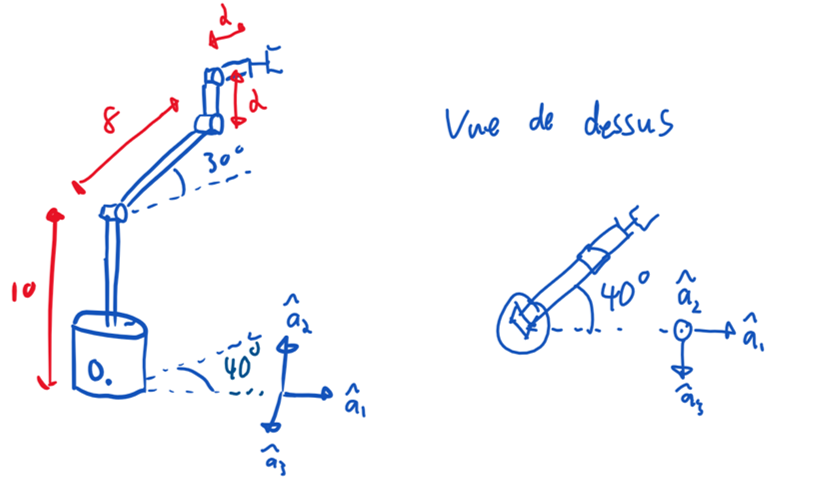
\includegraphics[width=0.65\textwidth]{exer_robot3D.png}
	\caption{Calcul de la cinématique d'un robot en 3D}
	\label{fig:exer_robot3D}
\end{figure}
%%%%%%%%%%%%%%%%%%%%%%

\paragraph{A)}
Identifier des points et bases vectorielles intermédiaires à utiliser. 

\paragraph{B)} 
Trouver le vecteur position de l'effecteur par rapport à l'origine $O$, exprimé dans la base vectorielle $a$.


%%%%%%%%%%%%%%%%%%%%%%%%%%%%%%%%%%%%%%%%%%%%%%%%%%%%%%%%%%%%%%
\section{Calcul de la cinématique d'une grue}

La figure \ref{fig:exer_grue3D} illustre une grue. 
%%%%%%%%%%%%%%%%%%%%%
\begin{figure}[H]
	\centering
		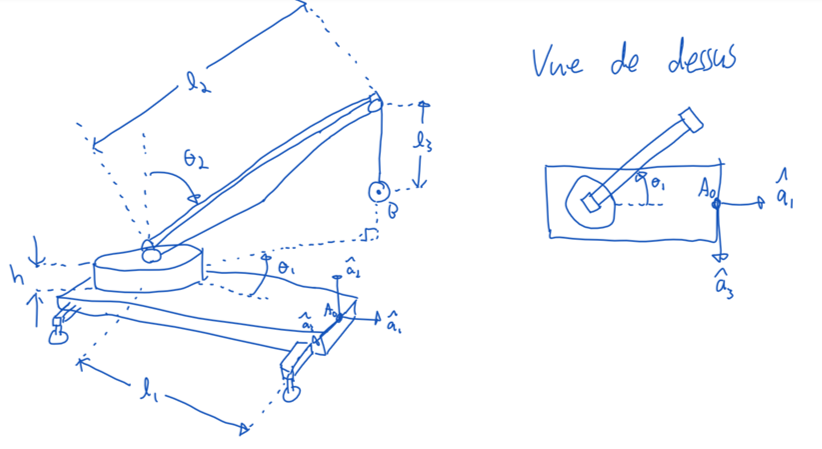
\includegraphics[width=0.75\textwidth]{exer_grue3D.png}
	\caption{Calcul de la cinématique d'un robot en 3D}
	\label{fig:exer_grue3D}
\end{figure}
%%%%%%%%%%%%%%%%%%%%%%

\paragraph{A)}
Identifier des points et bases vectorielles intermédiaires à utiliser. 

\paragraph{B)} 
Trouver le vecteur position du point $B$ par rapport à l'origine $A_o$, exprimé dans la base vectorielle $a$.




%%%%%%%%%%%%%%%%%%%%%%%%%%%%%%%%%%%%%%%%%%%%%%%%%%%%%%%%%%%%%%
\section{Calcul de la cinématique d'une jambe}

%%%%%%%%%%%%%%%%%%%%%
\begin{figure}[H]
	\centering
		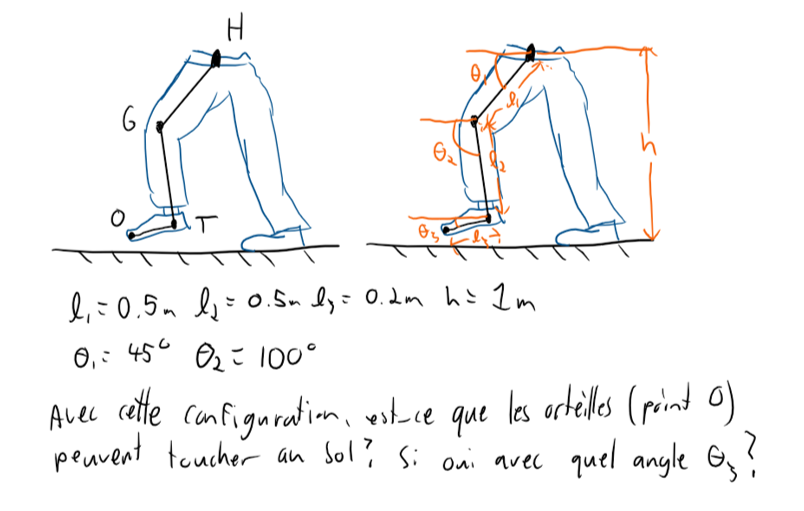
\includegraphics[width=0.75\textwidth]{exer_jambe.png}
	\caption{Calcul de la cinématique d'une jambe}
	\label{fig:exer_jambe}
\end{figure}
%%%%%%%%%%%%%%%%%%%%%%


%%%%%%%%%%%%%%%%%%%%%%%%%%%%%%%%%%%%%%%%%%%%%%%%%%%%%%%%%%%%%%
\subsection{Calcul de la cinématique d'un robot à trois joints}

%%%%%%%%%%%%%%%%%%%%%
\begin{figure}[H]
	\centering
		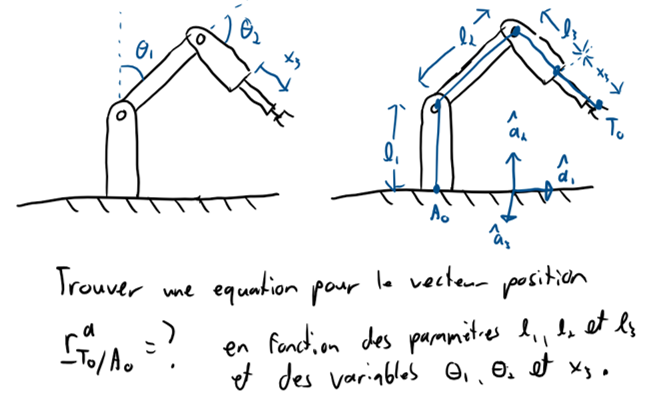
\includegraphics[width=0.75\textwidth]{exer_robot2D.png}
	\caption{Calcul de la cinématique d'un robot à trois joints}
	\label{fig:exer_exer_robot2D}
\end{figure}
%%%%%%%%%%%%%%%%%%%%%%